\chapter{Conductores y aislantes}\label{ch:g4:conductors-insulators}

¿Por qué son de metal los cables eléctricos --- pero van vestidos de
plástico? ¿Por qué conduce la corriente el puentecito del
\omterm{ex:g3:first-electric-circuit:switch}{interruptor} mientras su carcasa mantiene tus dedos a salvo? El año
pasado cerrábamos bucles; este año preguntamos por qué materiales
puede viajar la electricidad. La respuesta reparte todos los
materiales en dos clases: \omterm{def:g4:conductors-insulators:conductor}{conductores} y \omterm{def:g4:conductors-insulators:insulator}{aislantes}.

\section{El probador}

\begin{method}[Construir un probador]\label{met:g4:conductors-insulators:tester}
Construye el bucle del año pasado --- \omterm{def:g3:first-electric-circuit:battery}{pila}, cables, \omterm{def:g3:first-electric-circuit:bulb}{bombilla} ---
pero deja un hueco a propósito: dos puntas de cable libres, separadas
el ancho de un dedo.
\begin{enumerate}
  \item junta las dos puntas libres: la \omterm{def:g3:first-electric-circuit:bulb}{bombilla} se enciende ---
        el probador funciona;
  \item tiende sobre el hueco el objeto que quieras probar, con una
        punta de cable bien apretada contra cada extremo;
  \item mira la \omterm{def:g3:first-electric-circuit:bulb}{bombilla}: si hay \omterm{def:g1:light-and-shadows:source}{luz}, la electricidad ha
        atravesado el objeto; si hay oscuridad, no ha podido.
\end{enumerate}
La \omterm{def:g3:first-electric-circuit:bulb}{bombilla} da la respuesta: se enciende exactamente cuando el
objeto probado completa el bucle.
\end{method}

\begin{omfigure}
\begin{tikzpicture}[scale=0.9]
  \draw (0,0) to[battery1, l=pila] (0,2.6)
    to[short] (2.2,2.6)
    to[lamp, l=bombilla] (4.4,2.6)
    to[short] (6.0,2.6) -- (6.0,1.7);
  \draw (6.0,0.9) -- (6.0,0) to[short] (0,0);
  \fill (6.0,1.7) circle (1.6pt) node[right, font=\small]
    {~punta libre};
  \fill (6.0,0.9) circle (1.6pt) node[right, font=\small]
    {~punta libre};
  \draw[thick, fill=omMeth, fill opacity=0.4]
    (5.75,0.95) rectangle (6.25,1.65);
  \node[right, font=\small] at (6.6,1.3) {objeto probado};
\end{tikzpicture}

{\small El probador: un bucle sano con un hueco. Lo que tienda un
puente sobre el hueco es lo que se está probando --- la \omterm{def:g3:first-electric-circuit:bulb}{bombilla}
enseña si la corriente lo atraviesa.}
\end{omfigure}

\section{Conductores y aislantes}

\begin{definition}[Conductor]\label{def:g4:conductors-insulators:conductor}
Un \emph{conductor}\index{conductor} es un material que deja viajar la
electricidad por su interior. En el probador, un conductor que tiende
un puente sobre el hueco cierra el bucle y enciende la \omterm{def:g3:first-electric-circuit:bulb}{bombilla}.
\end{definition}

\begin{definition}[Aislante]\label{def:g4:conductors-insulators:insulator}
Un \emph{aislante}\index{aislante} es un material que le corta el paso
a la electricidad. Tender un puente sobre el hueco con un aislante
deja el bucle tan abierto como antes: la \omterm{def:g3:first-electric-circuit:bulb}{bombilla} se queda apagada.
\end{definition}

\begin{example}[Una mañana de pruebas]\label{ex:g4:conductors-insulators:trials}
Resultados de un probador de clase: un clip de acero --- \omterm{def:g1:light-and-shadows:source}{luz}. Una
moneda --- \omterm{def:g1:light-and-shadows:source}{luz}. Papel de aluminio de cocina --- \omterm{def:g1:light-and-shadows:source}{luz}. Una llave
--- \omterm{def:g1:light-and-shadows:source}{luz}. Una regla de plástico --- oscuridad. Un lápiz de madera ---
oscuridad. Una canica de vidrio --- oscuridad. Una goma de borrar ---
oscuridad. Una tira de papel --- oscuridad. El patrón salta a la
vista: los objetos que encienden la \omterm{def:g3:first-electric-circuit:bulb}{bombilla} son todos de metal.
\end{example}

\begin{proposition}[Los metales conducen]\label{prop:g4:conductors-insulators:metals}
Todos los metales conducen la electricidad --- el hierro, el cobre, el
aluminio, el oro, todos ellos ---, y por eso los remilgos del
\omterm{def:g1:magnets:magnet}{imán} con el hierro nos sorprendieron pero el probador no nos
sorprenderá nunca. Casi todos los demás \omterm{def:g3:solids-liquids-gases:solid}{sólidos} cotidianos --- el
plástico, la madera, el vidrio, la goma, el papel, la cera --- son
\omterm{def:g4:conductors-insulators:insulator}{aislantes}.
\end{proposition}

\begin{remark}[Conductor no es magnético]\label{rem:g4:conductors-insulators:notmagnet}
No confundas los dos talentos de los metales. El \omterm{def:g1:magnets:magnet}{imán} elige solo el
hierro y su familia; la corriente eléctrica es mucho menos exigente y
viaja por \emph{todos} los metales. El papel de aluminio que no le
hacía ningún caso a tu \omterm{def:g1:magnets:magnet}{imán} conduce la corriente de maravilla --- dos
juegos distintos, dos reglas distintas.
\end{remark}

\section{Conductores y aislantes trabajan juntos}

\begin{example}[Anatomía de un cable]\label{ex:g4:conductors-insulators:wire}
Mira la punta del cable de una lámpara justo donde entra en el
enchufe: por dentro corre cobre brillante --- un \omterm{def:g4:conductors-insulators:conductor}{conductor}, la
carretera de la corriente ---; a su alrededor se enrolla plástico de
color --- un \omterm{def:g4:conductors-insulators:insulator}{aislante}, la valla de la carretera. El cobre hace el
trabajo; el plástico mantiene la corriente dentro y tus dedos fuera.
Todos los cables de tu casa emparejan a los dos: un \omterm{def:g4:conductors-insulators:conductor}{conductor} dentro
de un \omterm{def:g4:conductors-insulators:insulator}{aislante}.
\end{example}

\begin{omfigure}
\begin{tikzpicture}[scale=0.85]
  \draw[thick, fill=omExo, fill opacity=0.25]
    (0.5,0.35) rectangle (6.5,1.65);
  \draw[thick, fill=omThm, fill opacity=0.45]
    (0.5,0.78) rectangle (7.6,1.22);
  \node[right, font=\small] at (8.35,1.8) {funda de plástico: aislante};
  \draw[-Stealth, omExo] (8.3,1.8) -- (6.3,1.55);
  \node[right, font=\small] at (8.35,1.0) {alma de cobre: conductor};
  \draw[-Stealth, omExo] (8.3,1.0) -- (7.72,1.0);
\end{tikzpicture}

{\small Un cable eléctrico desnudado: una carretera de cobre para la
corriente, dentro de una valla de plástico para la seguridad.}
\end{omfigure}

\begin{omfigure}
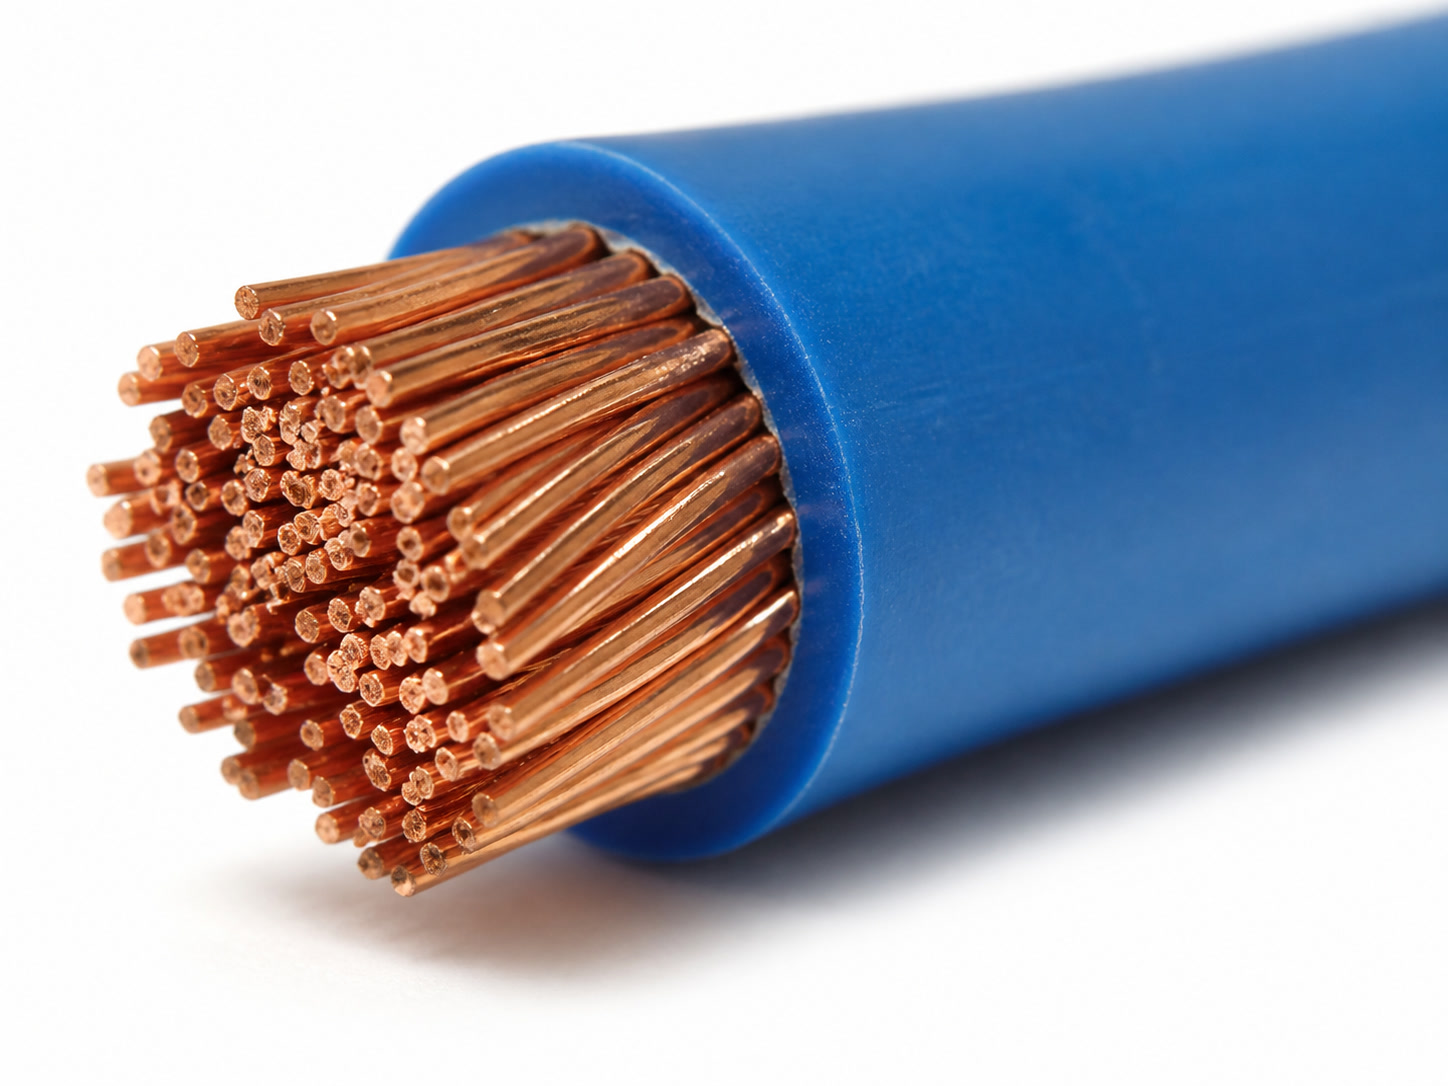
\includegraphics[width=0.5\linewidth]{images/book1/ai/g4-conductors-cable.jpg}

{\small La punta cortada de un cable, en la realidad: hilos de cobre brillante --- el \omterm{def:g4:conductors-insulators:conductor}{conductor} --- dentro de su funda de plástico de color --- el \omterm{def:g4:conductors-insulators:insulator}{aislante}.}
\end{omfigure}

\begin{example}[Leer los objetos de cada día]\label{ex:g4:conductors-insulators:objects}
Ahora muchos diseños se explican solos. El \omterm{ex:g3:first-electric-circuit:switch}{interruptor}: un puente de
metal (tiene que llevar la corriente) dentro de una carcasa de
plástico (tu dedo no debe llevarla). El destornillador del
electricista: hoja de acero, mango grueso y \omterm{def:g4:conductors-insulators:insulator}{aislante}. El enchufe:
metal en el fondo, plástico en la cara exterior. Las torres de alta
tensión llevan cables de metal desnudo altísimos y fuera del alcance,
colgados de largos discos \omterm{def:g4:conductors-insulators:insulator}{aislantes} para que la corriente no se cuele
hacia la torre.
\end{example}

\begin{remark}[El agua, las personas y por qué existen las reglas]\label{rem:g4:conductors-insulators:safety}
Hay que nombrar un \omterm{def:g4:conductors-insulators:conductor}{conductor} más: \emph{las cosas húmedas} ---
incluida la piel humana húmeda. Nosotros conducimos mal, pero el
enchufe de la pared empuja de manera tan tremenda que ``mal'' es más
que suficiente. Esta es la razón profunda de las normas de seguridad
que ya conoces: no meter nada en los enchufes, no tocar nunca nada
eléctrico con las manos mojadas, mantener los secadores lejos de la
bañera. El probador de \omterm{def:g3:first-electric-circuit:battery}{pila} no tiene peligro \emph{porque} el empuje
de una \omterm{def:g3:first-electric-circuit:battery}{pila} es diminuto; el enchufe no perdona nada.
\end{remark}

\section{Ejercicios}

\begin{exercise}[$\star$]\label{exo:g4:conductors-insulators:1}
¿Qué es un \omterm{def:g4:conductors-insulators:conductor}{conductor}? ¿Y un \omterm{def:g4:conductors-insulators:insulator}{aislante}? ¿Cuál de los dos
enciende la \omterm{def:g3:first-electric-circuit:bulb}{bombilla} del probador?
\end{exercise}

\begin{exercise}[$\star$]\label{exo:g4:conductors-insulators:2}
Reparte en \omterm{def:g4:conductors-insulators:conductor}{conductores} y \omterm{def:g4:conductors-insulators:insulator}{aislantes}: una cuchara de acero; \ un
corcho; \ papel de aluminio; \ un vaso de vidrio; \ una moneda de
cobre; \ una pieza de plástico.
\end{exercise}

\begin{exercise}[$\star$]\label{exo:g4:conductors-insulators:3}
Antes de cualquier prueba, ¿cómo compruebas que el propio probador
funciona? ¿Por qué es importante esta comprobación?
\end{exercise}

\begin{exercise}[$\star$]\label{exo:g4:conductors-insulators:4}
Un objeto de prueba deja la \omterm{def:g3:first-electric-circuit:bulb}{bombilla} apagada. Da dos razones
posibles --- una sobre el objeto y otra sobre una prueba mal hecha.
\end{exercise}

\begin{exercise}[$\star$]\label{exo:g4:conductors-insulators:5}
¿Por qué es de cobre por dentro y de plástico por fuera el cable de
una lámpara? ¿Qué trabajo hace cada material?
\end{exercise}

\begin{exercise}[$\star$]\label{exo:g4:conductors-insulators:6}
En un \omterm{ex:g3:first-electric-circuit:switch}{interruptor}, ¿qué parte es conductora y cuál \omterm{def:g4:conductors-insulators:insulator}{aislante}? ¿Por
qué necesita las dos?
\end{exercise}

\begin{exercise}[$\star$]\label{exo:g4:conductors-insulators:7}
El papel de aluminio no le hace ningún caso a un \omterm{def:g1:magnets:magnet}{imán}.
¿Encenderá la \omterm{def:g3:first-electric-circuit:bulb}{bombilla} del probador? ¿Qué regla responde y contra
qué confusión avisa la \cref{rem:g4:conductors-insulators:notmagnet}?
\end{exercise}

\begin{exercise}[$\star$]\label{exo:g4:conductors-insulators:8}
Un lápiz es madera con una mina de grafito. El probador de Nino se
queda apagado a través de la madera pintada, pero se enciende
débilmente de punta a punta a través del grafito afilado. ¿Qué ha
descubierto Nino sobre los dos materiales del lápiz?
\end{exercise}

\begin{exercise}[$\star$]\label{exo:g4:conductors-insulators:9}
¿Por qué tienen mangos gruesos de plástico los destornilladores y los
alicates de los electricistas? ¿Qué material protege a quién?
\end{exercise}

\begin{exercise}[$\star\star$]\label{exo:g4:conductors-insulators:10}
Una cadena de collar da ``\omterm{def:g1:light-and-shadows:source}{luz}'' en el probador; un collar de cuentas
de madera da ``oscuridad''; y un collar de cuentas de metal anudadas
en un cordón grueso de algodón da ``oscuridad'' también --- ¡aunque
todas las cuentas conducen! Explica el tercer resultado siguiendo la
carretera de la corriente de cuenta en cuenta.
\end{exercise}

\begin{exercise}[$\star\star$]\label{exo:g4:conductors-insulators:11}
¿Por qué es muchísimo más peligroso tocar cosas eléctricas con las
manos mojadas que con las manos secas? ¿Y por qué el probador de
\omterm{def:g3:first-electric-circuit:battery}{pila} no tiene peligro para tus experimentos mientras que el enchufe
lo tiene siempre? Usa la \cref{rem:g4:conductors-insulators:safety}.
\end{exercise}
